\title{\vskip -3cm \large \textbf{Introduction to a high-performance multi-period optimal power flow solver}}
\logo{%
    
\includegraphics[width=3cm,height=3cm,keepaspectratio]{ntnulogo_eng}~%
}

\author{Salman Zaferanlouei\\  \vskip 1cm \textbf{Winter School Workshop 2022}\\ Quality Hotel Skifer \\ Oppdal }

\begin{backgroundblock}{10mm}{25mm}
\begin{columns}
    \column{0.5\textwidth}
    \begin{figure}
 \begin{tikzpicture}
    \node[anchor=east,inner sep=0] (B) at (4,0) {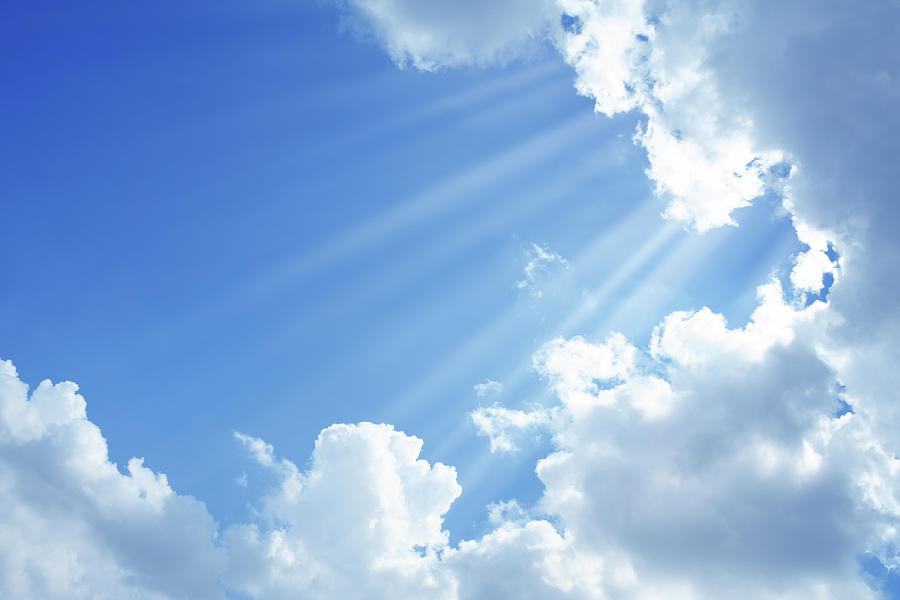
\includegraphics[scale=0.48]{Figures/cleansky.jpg}};
           \fill [draw=none, fill=white, fill opacity=0.5] (B.north west) -- (B.north east) -- (B.south east) -- (B.south west) -- (B.north west) -- cycle;
    \end{tikzpicture}
        \end{figure}
 \begin{figure}
 \begin{tikzpicture}
    \node[anchor=east,inner sep=0] (B) at (4,0) {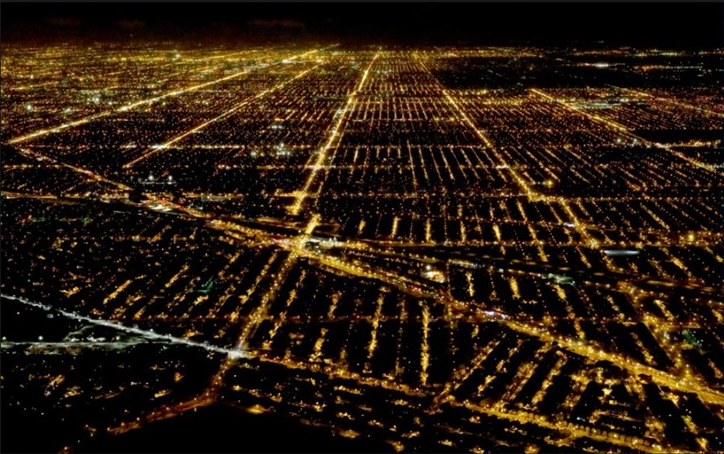
\includegraphics[scale=0.27]{Figures/title1.png}};
           \fill [draw=none, fill=white, fill opacity=0.5] (B.north west) -- (B.north east) -- (B.south east) -- (B.south west) -- (B.north west) -- cycle;
    \end{tikzpicture}
        \end{figure}

        \column{0.5\textwidth}
        \begin{figure}
  \begin{tikzpicture}
    \node[anchor=east,inner sep=0] (B) at (4,0) {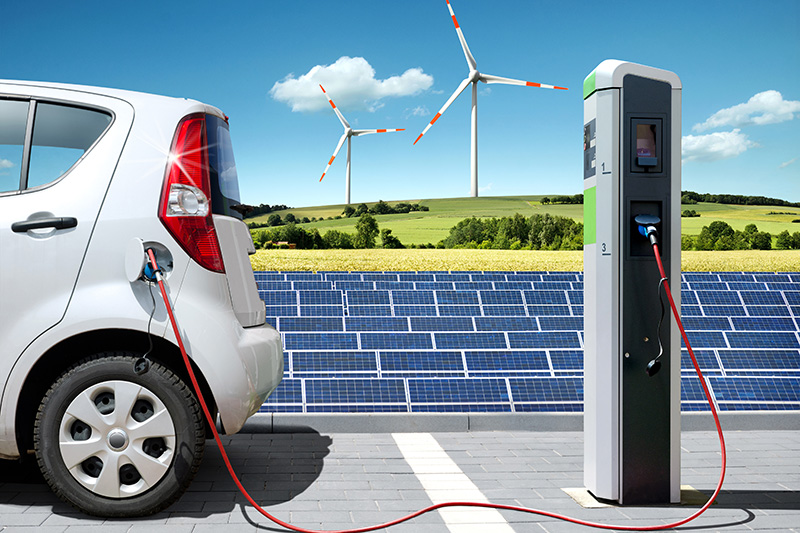
\includegraphics[scale=0.13]{Figures/EleV.jpg}};
           \fill [draw=none, fill=white, fill opacity=0.7] (B.north west) -- (B.north east) -- (B.south east) -- (B.south west) -- (B.north west) -- cycle;
    \end{tikzpicture}
\label{ComplexAdaptiveSystem}
        \end{figure}
 \begin{figure}
 \begin{tikzpicture}
    \node[anchor=east,inner sep=0] (B) at (4,0) {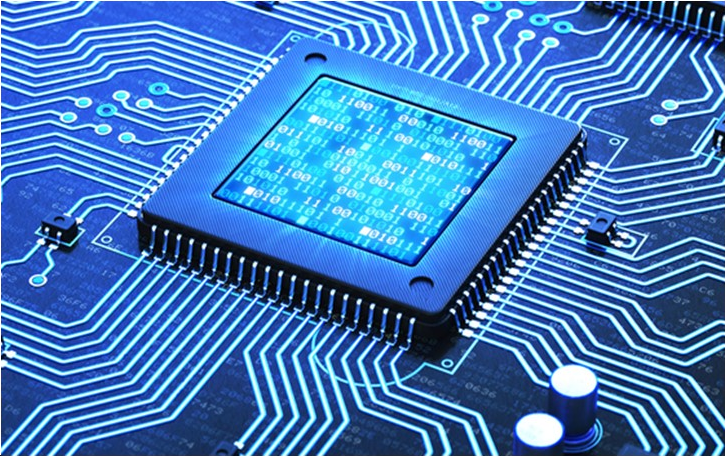
\includegraphics[scale=0.27]{Figures/title2.png}};
           \fill [draw=none, fill=white, fill opacity=0.5] (B.north west) -- (B.north east) -- (B.south east) -- (B.south west) -- (B.north west) -- cycle;
    \end{tikzpicture}
        \end{figure}

\end{columns} 
   \end{backgroundblock} 
\institute{{\\ }  \scalebox{1}{\insertlogo}}
\date{\vskip -1cm \small March 3, 2022}
